\section{Distributed Systems}
Distributed systems have emerged as the dominant execution environment for modern software systems~\cite{SteenTanenbaum2016}. They form the foundation of contemporary computing paradigms such as cloud infrastructures~\cite{Armbrust2010}, microservice architectures~\cite{Dragoni2017}, and Internet of Things (IoT) ecosystems~\cite{Atzori2010}. While these paradigms target different application domains, they share a common architectural principle: software functionality is realized through multiple distributed components that interact and coordinate over a network in order to accomplish a common task.

According to the seminal definition by van Steen and Tanenbaum~\cite{SteenTanenbaum2016}, a distributed system is a collection of autonomous computing elements that appears to its users as a single coherent system. These computing elements, often referred to as nodes or endpoints~\cite{Montesi2013}, execute concurrently and coordinate their actions by exchanging messages via communication channels, e.g., TCP/IP sockets~\cite{Braden1989}. Despite this internal distribution and concurrency, distributed systems aim to provide distribution transparency, hiding the underlying complexity so that users and applications perceive the system as a single unified entity~\cite{SteenTanenbaum2016}.

However, the scalability and autonomy that drive the adoption of distributed systems also introduce significant challenges. A key challenge is that, due to their autonomy, endpoints typically operate without a shared notion of time, such as a global clock~\cite{Lamport2019}. This lack of synchronization, combined with the non-deterministic behavior of concurrent executions, makes programming safe distributed software notoriously error-prone~\cite{Montesi2013}. Typical consequences of these complexities include safety issues such as $(i)$ deadlocks, where systems freeze due to indefinite waiting for messages~\cite{Coffman1971}, and $(ii)$ race conditions, where faulty computations occur due to uncoordinated access to shared resources~\cite{NetzerMiller1992}.

The challenge of ensuring safety is further amplified by the fact that traditional diagnostic techniques, such as testing and debugging, are often unreliable in concurrent settings~\cite{Bianchi2018}. Bugs frequently appear non-deterministically, making them difficult to reproduce and identify~\cite{McDowellHelmbold, Heisenbugs}. From a formal perspective, the concurrent execution of multiple programs leads to an exponential growth of possible execution traces, a phenomenon that complicates static analysis and verification~\cite{Montesi2013}. Consequently, the correctness of a distributed system depends heavily on the precise implementation of its communication flows.

\section{Choreographic Programming}
The paradigm of \textit{Choreographic Programming} was developed to address the inherent difficulty of coordinating separate endpoint programs. It aims to raise the level of abstraction for writing communication protocols by shifting the focus from individual node behavior to a global coordination plan, known as a \textit{choreography}~\cite{Montesi2023, CarboneM13}.

\subsection{Message-Passing Systems and the Endpoint Perspective}
%TODO Graphiken überarbeiten, evtl UML Diagramme
To understand the motivation behind choreographies, it is essential to first consider how communication is implemented in traditional distributed systems. In the message-passing paradigm, each endpoint is programmed from a local \textit{endpoint perspective}. Communication is realized through matching pairs of primitive operations: a \texttt{send} operation at one endpoint and a corresponding \texttt{receive} operation at another~\cite{Montesi2023}. 

\begin{figure}[h]
	\centering
	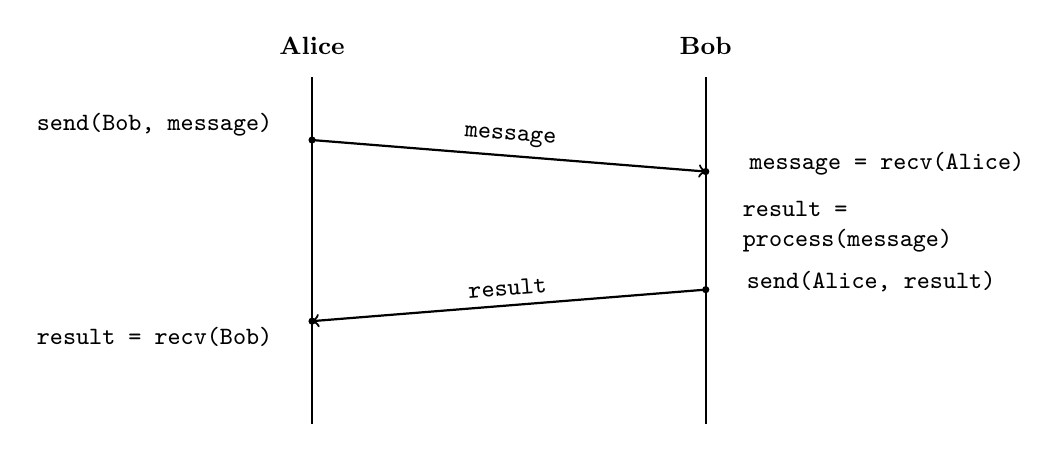
\begin{tikzpicture}[font=\small]
		% Participants
		\node (Alice) at (0,0) {\textbf{Alice}};
		\node (Bob) at (5,0) {\textbf{Bob}};
		
		% Lifelines
		\draw[thick] (0,-0.4) -- (0,-4.8);
		\draw[thick] (5,-0.4) -- (5,-4.8);
		
		% First message: Alice -> Bob
		\draw[->, thick] (0,-1.2) -- node[above, sloped] {\texttt{message}} (5,-1.6);
		\fill (0,-1.2) circle (1.3pt);
		\fill (5,-1.6) circle (1.3pt);
		
		% Bob local processing
		\node[align=left] at (6.8,-2.3) {\texttt{result =}\\ \texttt{process(message)}};
		
		% Second message: Bob -> Alice
		\draw[->, thick] (5,-3.1) -- node[above, sloped] {\texttt{result}} (0,-3.5);
		\fill (5,-3.1) circle (1.3pt);
		\fill (0,-3.5) circle (1.3pt);
		
		% Local actions
		\node[align=left] at (-2.0,-1.0) {\texttt{send(Bob, message)}};
		\node[align=left] at (7.3,-1.5) {\texttt{message = recv(Alice)}};
		\node[align=left] at (7.1,-3.0) {\texttt{send(Alice, result)}};
		\node[align=left] at (-2,-3.7) {\texttt{result = recv(Bob)}};
		
	\end{tikzpicture}
	\caption{Message Sequence Chart: Local view of communication between two participants Alice and Bob. Alice sends a message to Bob, Bob processes it locally, and then returns the result to Alice.}
	\label{fig:msc-alice-bob}
\end{figure}


As illustrated in \cref{fig:msc-alice-bob}, the overall interaction emerges only implicitly from the combination of independently developed local implementations. This requires programmers to manually ensure the proper alignment of actions across all nodes. In large-scale systems, managing these dependencies becomes increasingly difficult, as a missing \texttt{send} or a misaligned \texttt{receive} can lead to communication failures or deadlocks (see \cref{fig:mismatches}). Conceptually, developing systems from this perspective is \textit{akin to} writing in assembly, where developers must manually manage low-level communication states for every participant.
 \begin{figure}[h]
 	\centering
 	\begin{minipage}{0.46\textwidth}
 		\centering
 		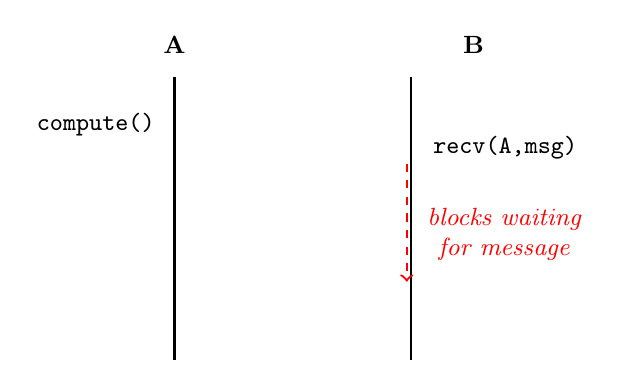
\begin{tikzpicture}[font=\small]
 			% Participants
 			\node (A) at (0,0) {\textbf{A}};
 			\node (B) at (3.8,0) {\textbf{B}};
 			
 			% Lifelines
 			\draw[thick] (0,-0.4) -- (0,-4.0);
 			\draw[thick] (3.0,-0.4) -- (3.0,-4.0);
 			
 			% A does something locally
 			\node[align=center] at (-1.0,-1.0) {\texttt{compute()}};
 			
 			% B waits for message
 			\node[align=left] at (4.2,-1.3) {\texttt{recv(A,msg)}};
 			
 			% Waiting marker
 			\draw[thick,red, dashed, ->] (2.95,-1.5) -- (2.95,-3.0);
 			\node[red, align=center] at (4.2,-2.4) {\textit{blocks waiting}\\\textit{for message}};
 			
 		\end{tikzpicture}
 		\caption*{(a) Blocking receive: B waits indefinitely for a message that A never sends}
 	\end{minipage}
 	\hfill
 	\begin{minipage}{0.46\textwidth}
 		\centering
 		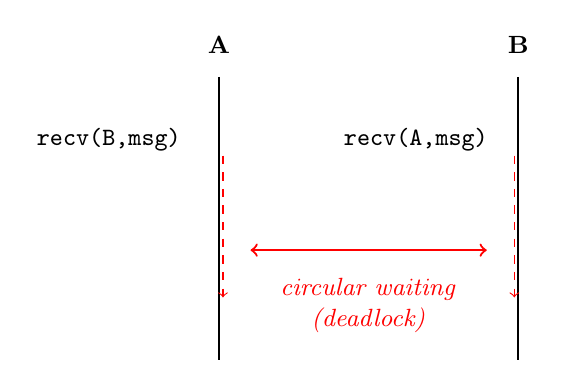
\begin{tikzpicture}[font=\small]
 			% Participants
 			\node (A) at (0,0) {\textbf{A}};
 			\node (B) at (3.8,0) {\textbf{B}};
 			
 			% Lifelines
 			\draw[thick] (0,-0.4) -- (0,-4.0);
 			\draw[thick] (3.8,-0.4) -- (3.8,-4.0);
 			
 			% Both try to receive first
 			\node[align=left] at (-1.4,-1.2) {\texttt{recv(B,msg)}};
 			\node[align=left] at (2.5,-1.2) {\texttt{recv(A,msg)}};
 			
 			% Waiting markers
 			\draw[red, dashed, ->] (0.05,-1.4) -- (0.05,-3.2);
 			\draw[red, dashed, ->] (3.75,-1.4) -- (3.75,-3.2);
 			
 			% Deadlock indication
 			\draw[red, <->, thick] (0.4,-2.6) -- (3.4,-2.6);
 			\node[red, align=center] at (1.9,-3.3) {\textit{circular waiting}\\\textit{(deadlock)}};
 			
 		\end{tikzpicture}
 		\caption*{(b) Deadlock: both endpoints wait for each other and neither can proceed}
 	\end{minipage}
 	\caption{Typical communication failures in local message-passing systems}
 	\label{fig:mismatches}
 \end{figure}
 


\subsection{The Concept of Choreographies}
Choreographies provide a way to address these limitations by providing a global description of the interactions between endpoints, often referred to as a bird's-eye view~\cite{Montesi2023}. In a choreography, a communication is represented as a single \textit{atomic interaction}, typically expressed in the ``Alice and Bob'' notation introduced by Needham and Schroeder~\cite{NeedhamSchroeder1978}:
\begin{center}
	\texttt{A.msg -> B.x}
\end{center}
This notation specifies that participant \texttt{A} communicates message \texttt{msg} to participant \texttt{B}, where it is stored in variable \texttt{x}. Unlike the endpoint perspective, this interaction is described in one place, ensuring that the send and receive actions are inherently consistent. 

A choreography reduces the complexity of $n$ interacting state machines to a \textit{single flow of discourse}. Since the early 2000s, choreographic languages have evolved from simple notations to expressive languages that include features such as local state manipulation, functions, and modularity~\cite{CruzFilipe2022, Montesi2023}. These advancements serve as the foundation for the programming paradigm discussed next.

\subsection{The Choreographic Programming Paradigm}
\label{subsec:choreographic_programming_paradigm}
Choreographic Programming elevates the concept of a choreography to an executable coordination plan. Instead of implementing separate programs for each node, the developer writes a \textit{unified, single program} for the entire system~\cite{AliKuper2023}. A significant advantage of this approach is that the system's logic can be \textit{read line by line}. This eliminates the need to mentally reconstruct the protocol by \textit{following the flow of control as it jumps from node to node}.

The most profound property of this paradigm is that choreographies are \textit{deadlock-free by design}~\cite{CarboneM13, Montesi2013}. Because communication is modeled as atomic interactions, it is structurally impossible to specify common errors like unmatched sends or receives. To illustrate this, consider the protocol for a vending machine in Listing~\ref{lst:vending_choreo}.

\begin{listing}[ht]
	\begin{minted}{text}
		if !VendingMachine.priceReached(amount, price) {
			User -> VendingMachine : coin
		}
		
		if VendingMachine.priceReached(amount, price) {
			if VendingMachine.inStock() {
				VendingMachine -> User : snack
			} else {
				VendingMachine -> User : refund
			}
		}	
	\end{minted}
	\caption{A minimal choreography specifying the interaction between a user and a vending machine.}
	\label{lst:vending_choreo}	
\end{listing}

In this plan, the logic of both participants is expressed within a single control flow. For instance, the second conditional is evaluated globally, which keeps the \texttt{User} and the \texttt{VendingMachine} synchronized. Assuming that the choreography satisfies the required well-formedness conditions, projection constraints, and well-branchedness assumptions, the \textit{else}-branch illustrates the intuition behind \textit{deadlock-freedom by design}: since the machine is specified to send a \texttt{refund}, the \texttt{User} is projected into a corresponding state in which receiving that message is possible.

\subsection{Endpoint Projection (EPP) and Compliance}
\label{sec:epp}

To execute a global choreography in a distributed environment, the specification must be translated into local code for each participating node. This is achieved through \textit{Endpoint Projection} (EPP), a formal transformation that mechanically derives a network of \textit{compliant} endpoint programs from a global coordination plan~\cite{Montesi2013}. As illustrated in Figure \ref{fig:epp_workflow}, this methodology shifts the burden of synchronization from the developer to the compiler toolchain, operationalizing the "bird's-eye view" of the choreography.

\subsection*{Formal Definition of EPP}
Formally, EPP is defined as a mapping $\llbracket \cdot \rrbracket$ that projects a choreography $C$ onto the set of process names $\text{pn}(C)$. The projection of $C$ on a specific process $r$, written as $\llbracket C \rrbracket_r$, returns the local process term specifying the actions $r$ must execute. For a basic interaction, the projection operator $\llbracket \cdot \rrbracket_r$ is defined recursively:

\begin{equation}
	\llbracket p \to q; C' \rrbracket_r = 
	\begin{cases} 
		q!; \llbracket C' \rrbracket_r & \text{if } r = p \text{ (Sender)} \\
		p?; \llbracket C' \rrbracket_r & \text{if } r = q \text{ (Receiver)} \\
		\llbracket C' \rrbracket_r & \text{if } r \notin \{p, q\} \text{ (Uninvolved)}
	\end{cases}
\end{equation}

By assigning send primitives ($q!$) to the sender, receive primitives ($p?$) to the receiver, and skipping interactions for uninvolved parties, EPP ensures that each node only executes code strictly necessary for its role. The complete distributed system, or \textit{network}, is then defined as the parallel composition of all individual projections: $\llbracket C \rrbracket = \prod_{p \in \text{pn}(C)} p[\llbracket C \rrbracket_p]$.

\begin{figure}[ht]
	\centering
	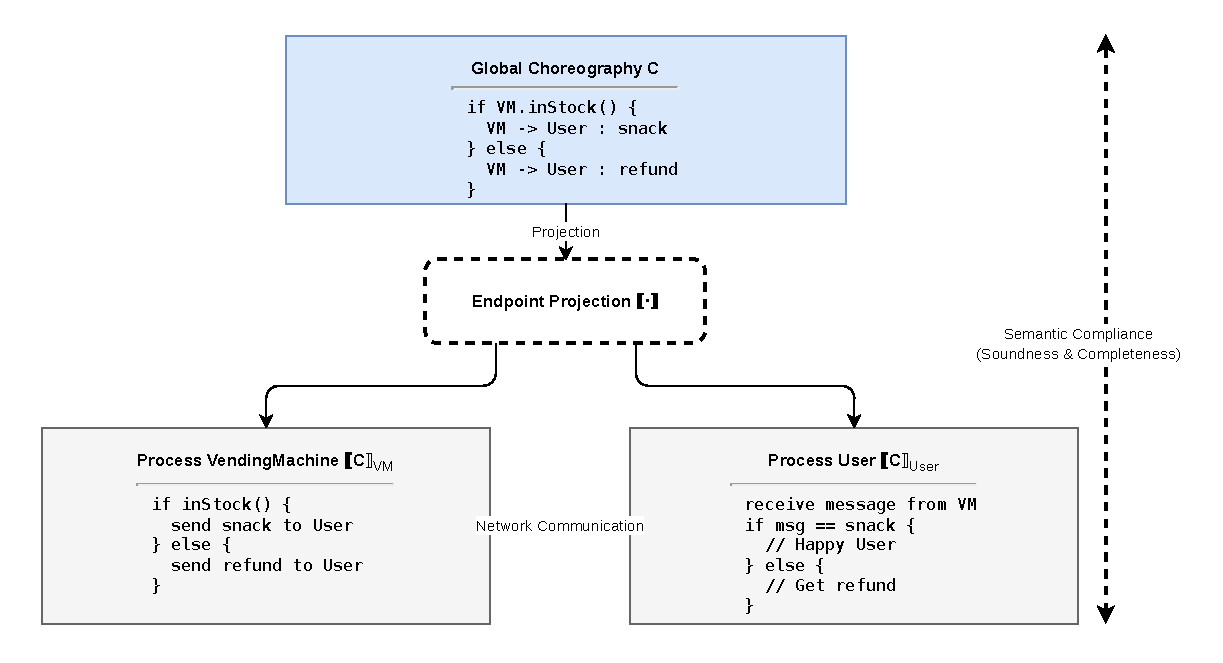
\includegraphics[width=\textwidth]{figures/EPP.drawio.pdf} 
	\caption{Workflow of Endpoint Projection: Decomposing a global choreography $C$ into compliant local terms $\llbracket C \rrbracket_p$.}
	\label{fig:epp_workflow}
\end{figure}

\subsection*{Correctness and Knowledge of Choice}
The central requirement for EPP is \textit{semantic preservation}, which ensures that the generated code faithfully implements the behavior specified in the choreography. This is formally expressed through two properties~\cite{Carbone2012}:
\begin{itemize}
	\item \textbf{Completeness:} The network can perform all transitions defined in the choreography ($C \xrightarrow{\mu} C' \implies \llbracket C \rrbracket \xrightarrow{\mu} \llbracket C' \rrbracket$).
	\item \textbf{Soundness:} The network performs \textit{only} those actions prescribed by the choreography ($\llbracket C \rrbracket \xrightarrow{\mu} N \implies \exists C': C \xrightarrow{\mu} C' \land N = \llbracket C' \rrbracket$).
\end{itemize}
Here, $\mu$ represents a transition label (signifying the interaction or action being performed), while $N$ denotes a network state, i.e., the parallel composition of process terms after a transition.

By satisfying these properties, EPP provides a formal basis for deriving endpoint implementations that are correct by construction and free from communication mismatches, deadlocks, and race conditions under the assumptions of the model. However, a critical challenge remains the \textit{Knowledge of Choice} (KoC) problem: when a choreography contains a conditional branch, the decision (e.g., a local check like \texttt{inStock()}) must be propagated to all affected participants to maintain global consistency~\cite{Montesi2023}. EPP therefore constitutes the central mechanism that connects global choreographic specifications to local distributed behavior and provides the deterministic foundation for the extensions considered in the following chapters.


\section{Markov Chains}
To quantitatively analyze the behavior of distributed systems under uncertainty -- such as communication delays, packet losses, or randomized algorithms -- purely deterministic models are insufficient. Instead, this thesis utilizes Markov chains as a mathematical foundation. A Markov chain is a stochastic process that satisfies the Markov property (memorylessness): the probability of transitioning to a future state depends solely on the current state and not on the history of previously visited states~\cite{Norris1997MarkovChains}. 

In the context of probabilistic model checking and tools such as PRISM, two primary variants are distinguished: $(i)$ Discrete-Time Markov Chains (DTMCs) and $(ii)$ Continuous-Time Markov Chains (CTMCs).

\subsection*{Discrete-Time Markov Chains}
Discrete-Time Markov Chains (DTMCs) model systems where transitions occur in discrete steps. They are particularly suitable for representing randomized algorithms or protocols where time is divided into fixed slots. 

Formally, a DTMC~\cite{Baier2008Principles} is defined as a tuple $\mathcal{D} = (S, s_{\mathit{init}}, P, L)$ where: 
\begin{itemize}
	\item $S$ is a finite set of states;
	\item $s_{\mathit{init}} \in S$ is the initial state;
	\item $P: S \times S \rightarrow [0, 1]$ is the transition probability matrix, such that $\sum_{s' \in S} P(s, s') = 1$ for all $s \in S$;
	\item $L: S \rightarrow 2^{AP}$ is a labeling function that assigns a set of atomic propositions ($AP$) to each state.
\end{itemize}

\paragraph{Example.}
As a simple example, consider a message transmission attempt. From an initial state $s_0$, the system moves to a success state $s_1$ with probability $0.9$ and to a failure state $s_2$ with probability $0.1$. The states $s_1$ and $s_2$ may be modeled as absorbing states, i.e., once reached, the system remains in them with probability 1. Formally, for the state order $(s_{0}, s_{1}, s_{2})$, the DTMC is given by the transition matrix
\[
P =
\begin{pmatrix}
	0 & 0.9 & 0.1 \\
	0 & 1   & 0   \\
	0 & 0   & 1
\end{pmatrix}.
\]

This illustrates the characteristic feature of a DTMC: the next state is chosen according to a discrete probability distribution over successor states.

In the context of this thesis, DTMCs serve as the semantic foundation to model the operational behavior of probabilistic choreographies. Within this framework, states represent global system configurations, while transitions capture atomic execution steps, such as message exchanges or probabilistic branching decisions. The transition probabilities are directly induced by the weights assigned to probabilistic choices within the choreographic specification. Consequently, DTMCs provide a rigorous basis for the quantitative analysis of protocols characterized by discrete-time behavior, such as the Peer-to-Peer protocol (\cref{sec:p2p}) and the Dining Cryptographers protocol (\cref{sec:dining-cryptographers}).


\subsection*{Continuous-Time Markov Chains}
While DTMCs are suitable for discrete steps, many distributed systems exhibit behavior that depends on continuous time, such as communication latencies or hardware failure rates. For these scenarios, Continuous-Time Markov Chains (CTMCs) are employed. 

A CTMC~\cite{Baier2008Principles} is formally defined as a tuple 
$\mathcal{C} = (S, s_{\mathit{init}}, R, L)$, where $S$, $s_{\mathit{init}}$, and $L$ are defined as in a DTMC, but:
\begin{itemize}
	\item $R: S \times S \rightarrow \mathbb{R}_{\ge 0}$ is the transition rate matrix.
\end{itemize}
The time spent in a state $s$ before a transition occurs follows an exponential distribution with the rate $E(s) = \sum_{s' \in S} R(s, s')$.

\paragraph{Example.}
As a simple example, consider a server that alternates between being idle and processing requests. Let $s_0$ denote the idle state, $s_1$ the processing state, and $s_2$ a failure state. From $s_0$, the server starts processing a request with rate $\lambda$. From $s_1$, it either completes the request and returns to $s_0$ with rate $\mu$, or it fails and moves to $s_2$ with rate $\theta$.
For the state order $(s_0, s_1, s_2)$, this yields the rate matrix
\[
R =
\begin{pmatrix}
	0 & \lambda & 0 \\
	\mu & 0 & \theta \\
	0 & 0 & 0
\end{pmatrix}.
\]
This illustrates the defining feature of a CTMC: transitions are governed by rates, which determine how quickly competing events occur in continuous time.

In contrast to DTMCs, CTMCs capture systems whose behavior depends not only on probabilistic branching, but also on the timing of events. This is particularly relevant for modeling real-time aspects of distributed systems, such as communication latencies or stochastic delays. In this thesis, CTMCs are used to analyze time- and performance-related properties, as demonstrated in the evaluation of the Modified Think Team Protocol (\cref{sec:think_team}).

In summary, DTMCs model probabilistic branching in discrete execution steps, whereas CTMCs capture stochastic behavior in continuous time through transition rates.
\section{The PRISM Model Checker}
To evaluate the efficiency and correctness of the choreographic language extension developed in this thesis, the PRISM model checker \cite{Kwiatkowska2018} is used as a primary reference and benchmarking tool. PRISM is a widely established framework for Probabilistic Model Checking (PMC), a formal verification technique used to analyze the likelihood of specific behaviors in stochastic systems. In this work, PRISM serves as a "gold standard" to validate that the state spaces generated by the choreographic projection are mathematically accurate and to provide a baseline for performance comparisons.

PRISM typically operates on high-level system descriptions written in its native PRISM modeling language. This state-based language organizes systems into modules that interact via shared variables and synchronized actions. When a user provides a PRISM model (e.g., a .pm file), the tool performs a process called state-space construction: it explores all possible configurations and transitions to build a global mathematical representation, such as a Discrete-Time Markov Chain (DTMC).

A central part of the evaluation in this thesis (see \Cref{ch:evaluation}) involves comparing the efficiency of this construction process. Specifically, we benchmark the runtime required by PRISM's native compiler to build a model against the time taken by our direct generation approach from choreographic specifications.

While PRISM is primarily used through its high-level language, it also provides an explicit interface for pre-constructed models. This interface allows external tools to bypass the PRISM compiler and provide the transition matrix directly. The explicit representation consists of three primary file formats:
\begin{itemize}
	\item \textbf{States Files (\texttt{.sta}):} An enumeration of all reachable global states.
	\item \textbf{Transitions Files (\texttt{.tra}):} A list of all transitions between states, including their associated probabilities (for DTMCs) or rates (for CTMCs).
	\item \textbf{Labels Files (\texttt{.lab}):} A mapping of states to atomic propositions for property verification.
\end{itemize}

The tool developed in this work is designed to generate these explicit formats directly. This enables a structural validation: by comparing the number of states and transitions in the .sta and .tra files generated by our tool with those generated by PRISM from an equivalent manual model, we can formally verify the correctness of the choreographic projection logic.

Although the core contribution of this thesis is the generation of models, the ultimate purpose of these models is their analysis. PRISM enables the verification of complex properties expressed in temporal logics, such as Probabilistic Computation Tree Logic (PCTL) for DTMCs and Continuous Stochastic Logic (CSL) for CTMCs. These logics allow for the calculation of:
\begin{itemize}
	\item \textit{Probabilities:} ``What is the likelihood that the protocol terminates within $N$ steps?''
	\item \textit{Expected Rewards:} ``What is the expected resource consumption (e.g., energy or time) until termination?''
\end{itemize}
By ensuring that our tool outputs PRISM-compatible explicit files, we provide a seamless path for users to utilize PRISM’s powerful numerical solvers for the downstream verification of generated choreographies.
